\apendice{Descripción de la adquisición y tratamiento de datos}

\section{Descripción formal de los datos}
El conjunto de datos utilizado en este trabajo procede del Servicio de Ginecología y Obstetricia del Hospital Universitario de Burgos (HUBU). Se trata de imágenes de ecografía obstétrica 2D correspondientes al corte transversal del cerebelo fetal, una vista estandarizada y clínicamente relevante para la evaluación de estas estructuras.

\subsection{Cohorte local}
Para el desarrollo del proyecto se planteó la utilización de un conjunto de imágenes procedentes del HUBU. La extracción de estas imágenes fue aprobada por el CEIM, en el marco del proyecto titulado "Detección de estructuras craneales en ecografías en distintas etapas del embarazo", cuyo dictamen favorable fue emitido el 6 de mayo de 2025 con número de registro CEIM 3246.

Tras su aprobación, el Servicio de Ginecología y Obstetricia del HUBU proporcionó las imágenes utilizadas en el proyecto, recopiladas en distintos periodos de tiempo. En total, se obtuvieron 198 imágenes, de las cuales 34 fueron seleccionadas como válidas para su uso en el estudio, atendiendo a criterios de calidad y adecuación anatómica. Esta selección garantizó el uso de los datos más representativos fueran incorporados al conjunto de entrenamiento.

Todas las pacientes incluidas en el estudio habían firmado previamente un consentimiento informado. No se realizó ninguna prueba adicional con fines exclusivos de investigación y todas las ecografías se llevaron a cabo como parte del seguimiento gestacional habitual, en el marco de atención clínica estándar.

El conjunto de datos utilizado en este proyecto, proporcionado por el HUBU y procesado para el entrenamiento del modelo, se encuentra alojado de forma interna en el repositorio de GitHub con el fin de permitir el despliegue de la aplicación. No obstante, dicho conjunto de datos no es entregado como parte del material físico del trabajo, en cumplimiento con la Ley Orgánica 2/2018, de 5 de diciembre, de Protección de Datos Personales y garantía de los derechos digitales, así como con las restricciones impuestas por el HUBU y el CEIM, que prohíben su cesión a terceros.

\subsubsection{Criterios de inclusión/exclusión}
Se incluyeron en el estudio mujeres embarazadas que acudieron a la Unidad de Ecografía Fetal del Servicio de Ginecología y Obstetricia del HUBU desde el 2 de septiembre de 2024 hasta el 9 de abril de 2025, ambos incluidos, para la realización de ecografías de cribado de malformaciones fetales en diferentes semanas de gestación, y que realizaron el control gestacional completo en dicho servicio y hospital. El equipo ecográfico empleado ha de ser: Voluson E-10 de General Electric, para evitar que diferentes softwares puedan proporcionar imágenes diferentes, debido al sistema de generación de la imagen. Asimismo, se seleccionaron embarazos con progenitores de etnia caucásica, con gestaciones de origen espontáneo (sin técnicas de reproducción humana asistida), simples (un solo feto).

Quedaron excluidas del estudio aquellas mujeres embarazadas que realizaran el seguimiento del embarazo fuera del HUBU, pero que acudieron a la Unidad de Ecografía Fetal del Servicio de Ginecología y Obstetricia del HUBU para una ecografía morfológica puntual. También se excluyeron del estudio los fetos con malformación fetal mayor, o que posean marcadores de aneuploidía en ecografía de la semana 12+0 - 13+6. Además, se excluyeron aquellos progenitores cuya etnia no fuera caucásica, así como gestaciones obtenidas mediante técnicas de reproducción humana asistida o múltiples. 

\subsection{Procesamiento y anotación del conjunto de datos}
La gestión y tratamiento de las imágenes ecográficas empleadas en el presente estudio se llevó a cabo a través de la plataforma Roboflow, que permitió:
\begin{itemize}
    \item La anotación manual precisa de las estructuras cerebelosas de interés.
    \item La creación de múltiples versiones del conjunto de datos conforme aumentaba el número de imágenes disponibles.
    \item La redimensión homogénea de las imágenes para facilitar su uso en el \textit{pipeline} de entrenamiento.
    \item La exportación de las anotaciones en formato COCO, lo que facilita la integración directa en el proceso de entrenamiento y evaluación del modelo.
\end{itemize}  

El conjunto final consta de 34 imágenes en formato \texttt{.jpg}, un número limitado debido a la dificultad de obtener imágenes ecográficas de alta calidad y bien anotadas. Esto justifica la segmentación manual y la puesta de bases para futuros desarrollos con conjuntos de datos más amplios. Las imágenes se distribuyen en tres subconjuntos: 26 se destinaron al entrenamiento, 4 para validación y 4 para el conjunto de prueba. A pesar del tamaño reducido del conjunto de datos, se priorizó la calidad de las imágenes y la precisión en su anotación para asegurar resultados fiables en el entrenamiento del modelo.

Las tres clases segmentadas son: \texttt{cerebelo} que agrupa ambos hemisferios cerebelosos, \texttt{la cisterna magna} y \texttt{vermis cerebeloso}. Esta agrupación se realizó para simplificar el modelo y reflejar la relevancia clínica de estas estructuras como unidades funcionales. Cada una de las imágenes fue revisada por personal médico especializado para garantizar la validez de las etiquetas aplicadas. 

La exportación en formato COCO facilita la centralización de todas las anotaciones en un único archivo JSON estructurado, donde cada entrada contiene información detallada sobre la imagen, las categorías de los datos segmentados y, segmentación para cada estructura de interés, facilitando la generación automática de máscaras de segmentación.

El flujo de procesamiento del proyecto ya incluye la organización automática de los conjuntos de entrenamiento, validación y prueba. Esto optimiza la fase de preparación de datos.
    
\section{Descripción clínica de los datos}

El cerebelo es una de las estructuras clave en la evaluación del neurodesarrollo fetal. Su estudio en la ecografía del segundo trimestre permite detectar anomalías estructurales que pueden estar asociadas a patologías neurológicas importantes, como el síndrome de Dandy-Walker o la hipoplasia cerebelosa.

Las estructuras seleccionadas para segmentación automática tienen una relevancia directa en la evaluación clínica:

\begin{itemize}
    \item \textbf{Vermis cerebeloso:} Estructura central que conecta ambos hemisferios. Su correcta formación es clave en el control del equilibrio, la postura y la coordinación motora \cite{wolf2009vermis}.
    \item \textbf{Cisterna magna:} Ubicada bajo el cerebelo, es un espacio lleno de líquido cefalorraquídeo que juega un papel importante en la circulación del LCR y en la evaluación neuroanatómica \cite{patel2023cisternamagna}. 
    \item \textbf{Cerebelo}: compuesto por los dos hemisferios cerebelosos que están involucrados tanto en la coordinación motora como en el aprendizaje de movimientos \cite{volpecerebelo}.
\end{itemize}
Estas estructuras son identificadas visualmente por parte del obstetra durante el estudio ecográfico, y su segmentación automática permite facilitar y estandarizar el diagnóstico clínico.

\begin{figure}[h]
    \centering
    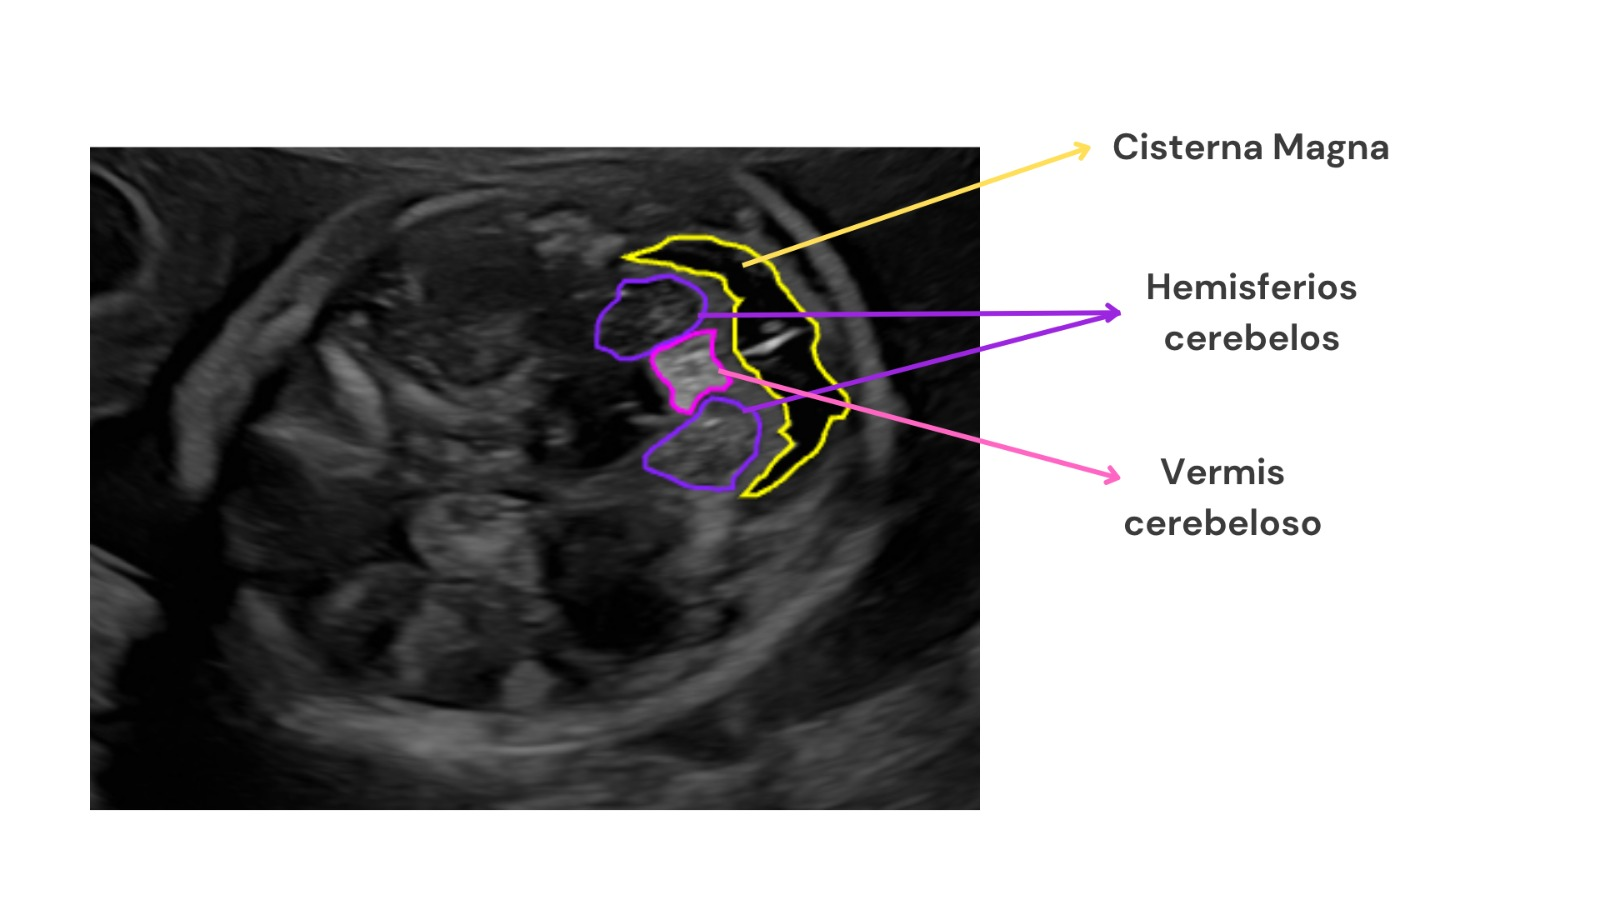
\includegraphics[width=0.8\textwidth]{img/estructuras_interes.jpeg}
    \caption{Localización de las principales estructuras del cerebelo.}
    \label{fig: parte_anatomicas_cerebelo}
\end{figure}
